\documentclass[11pt,a4paper]{article}
\usepackage[hyperref]{acl2020}
\usepackage{times}
\usepackage{tabularx}
\usepackage{latexsym}
\usepackage{graphicx}
\usepackage{subfig}
\renewcommand{\UrlFont}{\ttfamily\small}
\newcommand{\comment}[1]{\textcolor{red}{\bf \small [#1]}}
\newcommand{\spacemanidol}[1]{\textcolor{orange}{\bf \small [#1 --dc]}}
\aclfinalcopy 
\setlength\titlebox{5cm}
\newcommand\BibTeX{B\textsc{ib}\TeX}
\usepackage{microtype}
\aclfinalcopy 
\setlength\titlebox{5cm}
\newcommand\BibTeX{B\textsc{ib}\TeX}
\title{Can BERT Make Heads or Tails of Idioms? \\ Investigating Similarity between Idioms and Non-figurative Paraphrases in Contextualized Embeddings}
\author{Daniel Campos \And
  Paige Finkelstein \And 
    Elena Khasanova  \And
  Wes Rose  \And
  Josh Tanner }
\begin{document}
\maketitle
\begin{abstract}
Contextualized word embeddings produced by neural language models are now commonly used in paraphrase detection tasks, yielding state-of-the-art results. We use the task of paraphrase detection to investigate whether contextualized word embeddings encode information about idiom meaning and usage. We introduce a new dataset for paraphrase detection on sentences containing idioms, which we use in a series of fine-tuning and linear classification experiments. We also perform two vector similarity experiments, one on full sentence embeddings in conjunction with our paraphrase detection probing task and one that examines individual word embeddings in various contexts. We find that fine-tuned BERT is able to learn how to identify paraphrases containing idioms and that the contextualized embeddings are often sufficient input for our linear classifier to perform relatively well on the paraphrase detection task. We also show that while cosine similarity between sentence embeddings does not seem to be a useful diagnostic for paraphrase detection in sentences with idioms, contextualized word embeddings do contain semantic information capable of differentiating use of a word in an idiom phrase from its use in a literal context.
\end{abstract}


\section{Introduction}

The shift from using static, global word embeddings such as those produced by Word2Vec \cite{mikolov2013distributed} and GloVe \cite{Pennington2014GloveGV} to, instead, using contextualized word embeddings generated by neural language models such as ELMo \cite{Peters2018DeepCW}, GPT \cite{Radford2018ImprovingLU}, and BERT \cite{devlin2018bert} has been shown to yield state-of-the-art performance on a variety of NLP tasks \cite{devlin2018bert}. Accordingly, much recent work has made an attempt to understand the success of such models and to investigate whether, and how, these contextualized word embeddings encode various linguistic properties (\citet{Belinkov_2019}). We are interested in following in this vein of analysis to explore whether pre-trained language models are encoding semantic information about idiomatic language in their deeply contextualized embeddings, and whether this information can be used to identify similarity between an idiom and a non-figurative paraphrase. 

We deliver a few contributions to the field. First, we design a process for generating a novel idiom paraphrase dataset. Then, we perform a series of fine-tuning and linear classification experiments using this new dataset. We compare our results to performance on the Microsoft Research Paraphrase Corpus (MRPC) \cite{dolan-brockett-2005-automatically}, finding that BERT is able to perform comparably on our idiom paraphrase dataset. As an attempt to further explain BERT's performance on this task, we undertake a series of vector similarity experiments, both for word embeddings from individual words in context and for full sentence embeddings, with mixed results. Finally, we explain a few reasons that the high accuracy achieved on our dataset may not be fully representative of BERT's semantic understanding of idioms.\footnote{Our dataset and code is publicly available on Github at \href{https://github.com/spacemanidol/AnalyzingNeuralLanguageModelsGroup1}{https://github.com/spacemanidol/AnalyzingNeuralLanguageModelsGroup1}.}



\section{Related Work}
Paraphrase detection is a widely studied task in NLP. SemEval shared tasks often include paraphrase detection (\citet{Xu2015SemEval2015T1}; \citet{galbraith-etal-2017-talla}), and the GLUE benchmark collection contains several paraphrase and sentence similarity tasks \cite{wang2018glue}. Using contextualized word embeddings for paraphrase detection has become a common strategy (\citet{arase2019transfer}), and performance on MRPC is one of the state-of-the-art results cited in the original BERT paper (\citet{devlin2018bert}).
The representation and identification of idioms is also a subject that has received extensive treatment in NLP literature (\citet{Verma2015ANA}; \citet{liu-hwa-2018-heuristically}). As far as we are aware, however, our research is the first to focus specifically on investigating the treatment of idioms in the context of contextualized word embeddings.

\vspace{2mm}
\noindent\textbf{Paraphrase detection with metaphors} 

\noindent\citet{bizzoni-lappin-2018-predicting} propose a new corpus for a metaphor paraphrasing task and use it to test a deep neural network (DNN) on two paraphrase classification problems, showing that their model produces results that are significantly correlated with human judgments. In a follow-up study, they use this DNN to analyze the impact of additional context on metaphor paraphrase judgments \citep{bizzoni-lappin-2019-effect}. They find that, for both human judgments and the DNN's predictions, adding document context to the metaphor paraphrase task compresses scores toward the center of their paraphrase acceptability judgment scale. They explain, ``pairs that were given a very low score out of context tend to receive an increased score in context, while those with very high scores out of context decline in rating when presented in context" (173). 

We are also concerned with how context affects paraphrase detection in a non-literal context. Our research, however, incorporates the impact of context by exploring how contextualized word embeddings perform in a paraphrase detection probing task and evaluating the vector cosine similarity between word embeddings taken from idiomatic usages, literal usages, and paraphrase word usages.


\vspace{2mm}
\noindent\textbf{Probing Tasks with Multiword Expressions} 

\noindent \citet{shwartz2019pain} present an examination suite that includes six probing tasks related to lexical composition, and they compare results on this suite for six different models, concluding that contextualized word representations typically perform better than static word embeddings on these tasks. Their work focuses on comparing the performance of word embeddings from different models, and they examine both multiword expressions (as defined by \citet{10.5555/647344.724004} as ``idiosyncratic interpretations that cross word boundaries (or spaces)”) and also free word noun compounds and adjective-noun compounds. Our probing experiment is developed around the more general task of paraphrase detection, rather than tasks specifically focused on lexical composition such as recognizing verb-particle constructions. However, Shwartz and Dagan's experiments still provide a useful example of how to design a probing task in order to investigate how semantic meaning is captured in word embeddings across phrases.


\vspace{2mm}
\noindent\textbf{Vector similarity of contextualized embeddings} 


\noindent  One popular method for performing intrinsic evaluation of static word embeddings has been to examine the cosine similarity between vectors. However, this method of analysis has been criticized for several reasons, including the fact that there hasn't been compelling evidence of correlation between vector similarity and performance on extrinsic tasks such as paraphrasing or entailment \cite{faruqui-etal-2016-problems}. Yet despite such criticism, evaluation of vector similarity continues to be used as a method to investigate both static and contextualized embeddings. \citet{huang_cho_bowman_2020} use vector representations of words and their surrounding contexts to attempt to identify word senses from unsupervised data. \citet{ethayarajh2019contextual} measures cosine similarity between vectors in varying contexts at each layer of neural language models to conclude that  ``much like how upper layers of LSTMs produce more task-specific
representations (Liu et al., 2019a), upper layers of contextualizing models produce more context-specific representations" (56).

We build off of this tradition of examining differences in cosine similarity between vector representations in our current research in two ways. First, we add calculations of cosine similarity between sentences into our probing task experiments. Second, we carry out a supplemental experiment to examine the word-level embeddings, comparing the cosine similarity between words used in an idiom context, a literal context, a paraphrase usage, and a random word.

\section{Methods}
\subsection{Data Generation}
As we could find no suitable pre-existing dataset with idioms and their paraphrases, we created our own data for this task. Our dataset consists of 2000 sentence pairs, where the first sentence contains an idiom and the second sentence is either a paraphrase or non-paraphrase.

% I am not sure all these details should be given in the final paper, maybe just the sources and the final numbers?

To create our idiom paraphrase dataset, we start with idioms from the SLIDE \citet{Jochim2018SLIDEA} dataset and remove all idioms fewer than 3 words long. We then manually filter down to a set of 215 idioms using criteria based on linguistic diversity and our ability to generate paraphrases. We scrape examples containing these idioms from Reddit comments from 2011-08.\footnote{https://files.pushshift.io/reddit/comments/} From the 192,000 candidate comments, we filter down to a final set of 500 using criteria such as requiring that the idiom not be broken up. For each of the comments, we generate two paraphrases and two non-paraphrases.


We used two methods to produce candidate paraphrases. Half were written manually, and the other half were produced automatically and then manually reviewed. For some of our paraphrases, we replaced the idiom with another idiom.\footnote{To help with this, we scraped idioms from \href{https://idioms.thefreedictionary.com/}{The Free Dictionary’s Idioms} and \href{https://www.macmillandictionary.com/us/}{Macmillan Online English Dictionary}.}

For the non-paraphrases, we replaced the idioms either with hypernyms or hyponyms from Wordnet, antonymous expressions, or unrelated but distributionally expected expressions. Some examples of paraphrase candidates are shown as follows:

\vspace{2mm}
\begin{small}
\noindent\begin{tabular}{|p{\linewidth}|}
\hline
\textit{You're opening \textbf{a can of worms} you don't really want open.} \\\hline
Paraphrase (with an idiom): \textit{You're opening \textbf{a Pandora’s box} you don't really want open.}

\vspace{1mm}
Non-paraphrase (hypernyms/hyponyms): \textit{You're opening \textbf{a jar of centipedes} you don't really want open.}
\\\hline
\end{tabular}\\

\vspace{2mm}


\noindent\begin{tabular}{|p{\linewidth}|}
\hline \textit{I hope it has smaller \textbf{fish to fry}.} \\\hline
Paraphrase (with common language): \textit{I hope it has smaller \textbf{problems to deal with}.}

\vspace{1mm}
Non-paraphrase (opposite meaning): \textit{I hope it has \textbf{no problems}.} 

\vspace{1mm}
Non-paraphrase (unrelated): \textit{I hope it has \textbf{fried fish}.} \\\hline
\end{tabular}
\end{small}

The paraphrases have significant structural and lexical overlap with original sentences, which may have influenced the model performance to some extent. However, being aware of the issues raised in \citet{niven2019probing} and \citet{mccoy2019right} on unintentional bias in datasets, we kept the overlap consistent across the two labels (i.e. paraphrases and non-paraphrases) to reduce the potential for heuristics to develop in fine-tuning.\footnote{See \ref{section:dataset} in the appendix for further details.}

\subsection{Models}

Models for our idiom paraphrase classification experiments had two components: a base BERT model and a linear probe on top of the base BERT model. The linear probe was a single feed-forward linear layer,\footnote{\label{probe-wrong-note}Our classification layer was constructed and trained like a linear regression, with no final sigmoid and MSE for loss.} which was trained per experiment. We used a total of four BERT models: 1. \textit{bert-base-uncased}  as provided by the original authors, 2. fine-tuned on our data shuffled randomly, 3. fine-tuned on a ``disjoint'' subset of our data where each idiom appeared exclusively in train or test, and 4. fine-tuned on MRPC.

\subsection{Fine-Tuning}

We performed fine-tuning for the BERT models using the Transformers library \cite{Wolf2019HuggingFacesTS}. BERT's output for the sentence is passed through a ``pooling" layer which selects only the embedding for the CLS token, which is then fed through a single feed-forward layer and finally into a linear classification layer. This linear neural network has a hidden size of 768 and has dropout set to 0.1. Our input is two sentences separated by the SEP token, and since we are only outputting 0 or 1 the task is essentially a logistic regression. The output of this linear classifier ultimately determines the label, and because it is exclusively dependent on the content of the CLS token embedding, we can expect that fine-tuning will primarily effect the CLS embeddings. This is reflected in our linear probe classification results in Chart \ref{fig:accuracyByParadigm}. For all our fine-tuning, we kept the hyperparameters constant.\footnote{We use \textit{bert-base-uncased}, a batch size of 8, a learning rate of 5e-5, no weight decay, an adam epsilon of 1e-8, and we train for 10 epochs, evaluating the model every 100 steps.}



\subsection{Linear Probe}

\noindent In order to measure BERT's understanding of idioms, we evlauated its performance in classifying paraphrases across our data for several combinations of BERT models and hyperparameters. 

Our method for classifying paraphrases is as follows: obtain BERT embeddings, combine them into a single representative classification vector, and then use that as input to our linear probe. We experimented with multiple ways of producing representative classification vectors, which we call ``embedding paradigm" and designate as a hyperparameter of our experiments. For the embedding paradigm, we use either \textit{cls} or \textit{combined}. For \textit{cls}, we pass both sentences into BERT separated by the SEP token. We then simply select the embedding corresponding to the CLS token from the top layer. For \textit{combined}, we pass each sentence into BERT separately. We then produce ``sentence embeddings" from each sentence by taking an average of all of the word embeddings in each sentence, and then finally perform vector subtraction (subtracting the second from the first) to obtain a single vector to be passed to the linear probe. 

For a single trial, we select one of the four BERT models described above, a training dataset, a test dataset, and an embedding paradigm. We train only the linear probe, keeping the parameters of the BERT model frozen. Then we test using the test data. Our hyperparameter tuning was done experimentally, with our final hyperparameters being the ones that consistently performed well. Hyperparameters except embedding paradigm were then held static across all our experiments.\footnote{More on hyperparameters in section \ref{section:probehyper} of the appendix.}

As the \textit{cls} and \textit{combined} paradigms delivered significantly different results in many scenarios, we ran all of our experiments using both. We also experimented with a third embedding paradigm designed to more closely mimic the classification process used by the Transformers fine-tuning scripts \cite{Wolf2019HuggingFacesTS}, where we passed the CLS token embedding through a final feed-forward layer and used that as input to the linear probe. We found that this paradigm performed almost identically to the \textit{cls} paradigm, and so we restrict our reporting to the \textit{cls} and \textit{combined} paradigm embeddings.

\subsection{Embedding Vector Similarity}

We incorporate an analysis of vector cosine similarity into our research by comparing sentence embedding vectors for data used in the probing task and, more rigorously, by creating a secondary experiment to evaluate similarity between embeddings for words used in various contexts.

\vspace{2mm}
\noindent \textbf{Probe Task Sentence Embeddings}

 \noindent 
 For each sentence pair in the data used to train and test the probing classifier, we calculate the sentence embeddings by taking an average across all of the word embeddings in a sentence, and then calculate the cosine similarity between the two sentence embeddings. We also calculate the average cosine similarity between all paraphrase sentence pairs and all non-paraphrase sentence pairs, as well as the averages across each classification result category (i.e.  correctly predicted paraphrases, incorrectly predicted paraphrases, correctly predicted non-paraphrases, and incorrectly prediction non-paraphrases) for each run of the probe.

\vspace{2mm}
\noindent \textbf{Word Embedding Context Comparisons}

\noindent In order to further explore whether contextualized word embeddings encode information about the semantics of idioms, we perform an experiment that compares the vector representations for idiom words used in several different contexts. Specifically, we craft a dataset based around 30 common idioms. For each of these idioms, we identify one word that is a key word in the idiom (i.e. not a common stop word). We then construct a set of 25 sentences around each idiom phrase and key word in the phrase. Five of the sentences use the \textit{idiomatic phrase} itself, and many of these are taken from the dataset that we use in the probing task. Ten sentences use the key word from the idiom phrase in a \textit{literal} way. We also determine a \textit{paraphrase word} that represents the meaning of the key word in the idiom context, and obtain ten sentences that use this paraphrase word literally. As an example, starting with the \textit{idiom phrase} ``on the other hand," we designate  ``hand" as the \textit{key word} and ``perspective" as the \textit{paraphrase word} for this idiom key word in context. Then we generate sentences such as the following:

\vspace{1mm}

\begin{small}
\noindent\begin{tabular}{|p{\linewidth}|}
\hline
\textit{idiom usage sentence}: ``On the other hand, it is kind of distracting." \\\hline
\textit{literal usage sentence}: ``I count 11 scars on this hand." \\\hline
 \textit{paraphrase word sentence}: ``I think that most people that have seen the world will agree with your perspective." \\\hline
\end{tabular}\\
\end{small}

 We also add some groups of ten sentences using a random word, such as ``keyboard" or ``market" to use as a control group in the comparisons.\footnote{In addition to using the probing task data to obtain sentences, we use the \href{https://www.english-corpora.org/coca/}{Corpus of Contemporary American English} and  \href{https://www.macmillandictionary.com/us/}{Macmillan Online English Dictionary}.}

For each idiom phrase data group, we obtain a word embeddings for every word in each sentence by feeding the sentences, one at a time, into BERT. We run trials using four different BERT models: 1. \textit{bert-base-uncased} not fine-tuned, 2. \textit{bert-large-uncased} not fine-tuned, 3. \textit{bert-base-uncased} fine-tuned on MRPC, and 4. \textit{bert-base-uncased} fine-tuned on our idiom paraphrase dataset used for the probing task. Once we have the set of word embeddings for all of the sentences, we perform pairwise comparisons of the cosine similarity between the relevant word embedding in each sentence across each of the usage categories (idiom usage, literal key word usage, and paraphrase word usage). Here, for example, are the cosine averages for the data group built around the idiom phrase ``bite the bullet," using the non fine-tuned \textit{bert-base-uncased} to calculate word embeddings. The idiom \textit{key word} is ``bullet" and the \textit{paraphrase word} is ``situation."

\vspace{2mm}
\noindent
\begin{small}
\begin{tabular}{ |p{5.9cm}|p{1cm}|  }
\hline
\multicolumn{2}{|c|}{Word Embedding Average Cosine Similarities } \\
\hline
``bullet" in \textbf{idiom} usage v. \textbf{idiom} usage & 0.7999 \\
\hline
``bullet" in \textbf{idiom} usage v. \textbf{literal} usage & 0.5115 \\
\hline
``bullet" in \textbf{literal} usage v. \textbf{literal} usage & 0.6093 \\
\hline
``bullet" in \textbf{idiom} usage v.  ``situation" & 0.2612 \\
\hline
``bullet" in \textbf{literal} usage v. ``situation" & 0.2795 \\
\hline
``bullet" in \textbf{idiom} usage v. \textbf{random} word (``phone") & 0.3270 \\
\hline
\end{tabular}
\end{small}
We then also compute the average differences between each comparison category over the entire corpus of idiom phrase groups (30 groups total). Finally, we also use PCA to visualize similarity between the word embeddings calculated for each group.\footnote{For a sample of the PCA visualizations, see section \ref{section:pcaviz} in the appendix.} We perform PCA for three different combinations per idiom phrase group, namely:

1. idiom usage sentences (5) + literal usage sentences (10)

2. \#1 + paraphrase word sentences (10)

3. \#2 + random word sentences (10)

\section{Results}
\subsection{Fine-Tuning Results}
We ran 21 fine-tuning experiments seeking to explore how BERT performed on our dataset when we varied the source (MRPC, manually created, automatically created), training time, training size, and evaluation task.\footnote{Full results shown in Table \ref{tab:paraphraseFineTuneResultTable_Appendix} in the appendix.} We find that when BERT only has to optimize to a manually created or automatically created idiom paraphrases, it quickly reaches perfect or near perfect performance.\footnote{Full results shown in Figure \ref{fig:F1FineTuneSource} in the appendix.} This provides good evidence for the importance of varying dataset construction methods. We also find that, more so than on other paraphrase tasks, on our idiom paraphrases BERT performance varies widely based on the number of samples.\footnote{Shown in Figure \ref{fig:F1FineTunedataset} in the appendix.} We hypothesize that the diversity of our data and the high lexical and structural overlap in our paraphrase candidates makes learning idiom paraphrases more difficult. Finally, we find that BERT can transfer knowledge of paraphrase detection from our idiom paraphrase dataset to MRPC quite well, but results do not improve much with further fine-tuning.\footnote{The effectiveness of transfer learning across paraphrase tasks can be seen in Figure \ref{fig:F1FineTunetransfer} in the appendix.} Overall, we find that BERT does relatively well on our idiom paraphrase dataset, with a top result of 81.85\% when trained on all of our idiom data. 
% In this section we present results for the experiments described in section 3.3. We present our results in four sections to highlight some interesting findings.

\subsection{Linear Probe Results}


\begin{table*}[h]
\centering
\label{table1}
\begin{small}
\begin{tabular}{|l|l|l|l|l|} \hline
\textbf{Fine-Tune Data} & \textbf{Train Data} &  \textbf{Accuracy} & \textbf{F1} \\ \hline
Idiom Training Data  &Idiom Training Data & 78.50\% &78.60\% \\ \hline
Non Fine-tuned  &Idiom Training Data& 74.25\%&74.10\% \\ \hline
MRPC Training Data &Idiom Training Data&73.00\%&72.73\% \\ \hline
MRPC Training Data &MRPC Training Data&53.25\%&68.25\% \\ \hline
Non Fine-tuned &MRPC Training Data&52.00\%&67.90\% \\ \hline
Idiom Training Data &MRPC Training Data&51.50\%&67.78\% \\ \hline
\end{tabular}
\end{small}
\caption{Results on Idiom Paraphrase Task for model tested on idiom-data-all-dev, using \textit{combined} paradigm}
\label{tab:paraphraseResultTable}
\end{table*}
 Our best accuracy on the paraphrase probing classification task was 78.5\% using the \textit{combined} embedding paradigm, followed fairly closely by 77.8\% using the \textit{cls} embedding paradigm. In both cases, we fine-tuned BERT and trained on our own idiom data. Compared to the 80.6\% we achieved on MRPC using the \textit{cls} paradigm, this suggests that the idiom paraphrase task is not substantially more difficult than normal paraphrase detection, and that the task can be learned by BERT.
 
\begin{figure}[h]
    \includegraphics[width=8cm]{Paper/accuracyByParadigm.png}
    \centering
        \caption{Accuracy by Embedding Paradigm for a selection of fine-tuned models.  All models trained and tested on idiom data.}
    \label{fig:accuracyByParadigm}
\end{figure} 
 
 
 Figure \ref{fig:accuracyByParadigm} shows performance by embedding paradigm for each of the BERT models we used. The \textit{combined} embedding paradigm performs well consistently across the three BERT models, while the performance of the \textit{cls} embedding paradigm is highly dependent on the model, suggesting that the \textit{cls} paradigm is more representative of what the BERT model is learning via fine-tuning. Finally, an exploration of accuracy by epoch for BERT fine-tuned on our data and on MRPC shows that while fine-tuning on MRPC does help performance on our idiom paraphrase task, BERT fine-tuned on MRPC not only peaks at a lower accuracy (as one would expect), but also takes longer to achieve its maximum accuracy.\footnote{This can be seen in Figure \ref{fig:accuracyByEpoch} in the appendix.}
 
 Consider Table \ref{tab:paraphraseResultTable}, which shows performance on our idiom data when varying the fine-tuning data and the training data. The arguably most surprising result is that fine-tuning on our idiom paraphrase dataset and training the linear probe on MRPC produced performance just above chance. This suggests that while BERT may learn something transferable between MRPC and our data, the linear classification layer does not. 

Finally, to test whether the model having seen an idiom in training (either during fine-tuning or probe training) might influence its ability to understand the idiom during test, we ran a set of experiments mirroring our primary experiments, but using this our disjoint data set. We can see from Chart \ref{fig:accuracyByDataSplit} that performance on the disjoint data is slightly worse, though not to the extent that one might expect. 


\subsection{Vector Similarity Results}

\subsubsection{Probing Task Sentence Embeddings}
We hypothesized that there might be strong trends in sentence embedding cosine similarity across paraphrases and non-paraphrases and across the linear classifier's predictions. Overall, this did not seem to be the case. However, we did observe patterns in a couple specific experimental settings in which the average cosine for paraphrases was distinctly higher than that of non-paraphrases. Further, the averages across true positives and across true negatives had even more extreme values, while the false negatives and false positives were closer together. This was true of the model fine-tuned on MRPC and trained and tested on our idiom paraphrase data, as well as the non-fine-tuned model trained and tested on MRPC. However, as these results appeared to be outliers, more work would need to be done do determine if there are specific conditions where cosine similarity becomes a factor in classification.\footnote{Table \ref{tab:AvgCosineSimLinearClass} in the appendix shows detailed results.}

\noindent
\subsubsection{Word Embedding Context Comparisons}


If the cosine similarity scores are indeed highly correlated strictly with semantic meaning, we might expect to see results where the \textit{idiom usage} word and \textit{paraphrase} word's cosine similarity are higher than that between the \textit{idiom usage} and \textit{literal usage}. For example, the embedding for ``sack" in ``Soon we're going to hit the sack." would have higher cosine similarity with the embedding for ``bed" (\textit{paraphrase} word) in ``Stay in bed." than ``sack" in ``A sack of rice now costs \$18 in U.S. dollars." However, this is not what we observed. We instead find that the \textit{literal} usage and \textit{idiom} usage of the same word have a higher cosine similarity in almost all cases than the \textit{idiom} usage word and \textit{paraphrase} word, as show in Table \ref{tab:cosinesimcat}.\footnote{For all four of the models that we used to generate the word embeddings (\textit{bert-base-uncased} not fine-tuned, \textit{bert-large-uncased} not fine-tuned,  \textit{bert-base-uncased} fine-tuned on the MRPC, and \textit{bert-base-uncased} fine-tuned on our idiom paraphrase dataset), we observe the same trends in cosine similarity comparisons across the usage categories, so we only display the \textit{bert-base-uncased} results here.}


\begin{table}[htbp]
\caption{Cosine Similarity Category Comparisons}
\label{tab:cosinesimcat}
\begin{small}
\resizebox{\columnwidth}{!}{\begin{tabular}{|l|l|}
\hline
Usage Types &  Average Cosine Similarity  \\
\hline
idiom  v. idiom  & 0.7697  \\
literal v. literal  & 0.6546  \\
idiom v. literal  & 0.5223  \\
idiom v. paraphrase  & 0.3272  \\
literal v. paraphrase  & 0.3053 \\
\hline
\end{tabular}}
\end{small}

\end{table}


However, the results still suggest that the cosine similarity score is capturing some information about idiom usages of a word versus literal usages of the same word. We see that across all of the models, the average cosine similarity is highest between two words used in the same \textit{idiom context} in different sentences such as ``sack"  in ``Soon we're going to hit the sack." and ``Would it be okay with you if we had a bite to eat now and hit the sack early?" Furthermore, this cosine similarity between \textit{idiom} usage words is noticeably higher than the cosine similarity between \textit{idiom} usage words and the same word in \textit{literal} contexts, as shown in Table \ref{tab:idiomlit}.\footnote{Section \ref{section:cosinesimdiff} in the appendix further illuminates this trend by showing the average advantage of idiom v idiom usages over idiom v literal usages.} 

\begin{table}[htbp]
\caption{Idiom/Literal Pair Cosine Similarity}
\label{tab:idiomlit}
\resizebox{\columnwidth}{!}{\begin{tabular}{|l|l|1|}
\hline
Model &  idiom v idiom &  idiom v literal\\
\hline
\textit{bert-base-uncased} & 0.6546 & 0.7697\\
\textit{bert-large-uncased} & 0.7572 & 0.8153 \\
MRPC fine-tuned &   0.5889  & 0.6892\\
idiom paraphrase data fine-tuned  & 0.8226 & 0.6806\\
\hline
\end{tabular}}
\end{table}



\vspace{2mm}
\noindent \textbf{PCA Visualizations}

Examining the PCA visualizations produced for each idiom phrase group also suggests that the word embeddings contain semantic information about differences in idiom and literal usage.\footnote{All of the PCA images are available in the output folder for each run in our Github repo \href{https://github.com/spacemanidol/AnalyzingNeuralLanguageModelsGroup1/tree/master/vector_similarity/output}{here}. We also present them in this \href{https://github.com/spacemanidol/AnalyzingNeuralLanguageModelsGroup1/blob/master/vector_similarity/run_vector_similarity_words_comparison.ipynb}{Jupyter Notebook} for easier comparison.} In nearly every single PCA visualization of the data combination of word embeddings from idiom use sentences and literal use sentences, the two categories are cleanly and clearly divided. Figure \ref{fly} shows a randomly selected example that shows a randomly selected PCA visualization.\footnote{Embeddings produced from the model trained on our idiom paraphrase dataset.}

\begin{figure}[h]
\caption{Embeddings for the word ``fly'' used literally and used as part of the idiom ``on the fly"}
\label{fly}
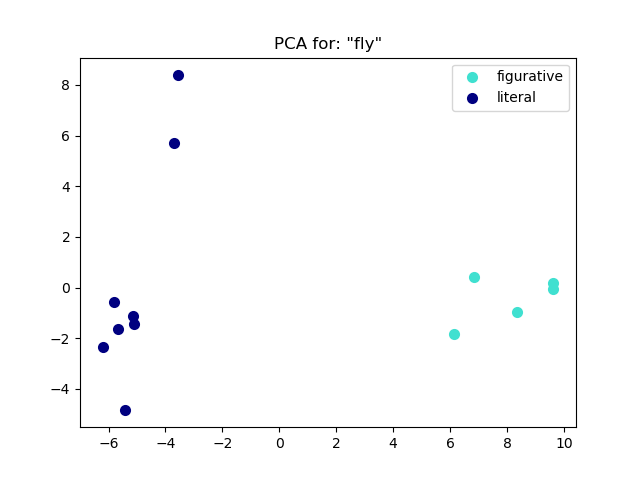
\includegraphics[height=5.5cm]{Paper/pair_id_22_fig_lit.png}
\end{figure}

The PCA visualizations across the data combinations that include the paraphrase sentences and random sentences also mostly maintain this division between the literal and idiom usages. Though sometimes the literal usage and idiom usage groups become mixed together with the paraphrase word and random word groups remaining distinct. 

We found that out of the four models used for producing the word embeddings, that the  non-fine-tuned \textit{bert-large-uncased} model embeddings produced PCA visualizations that kept the idiom usage and literal usage contexts most clearly divided, while the model fine-tuned on MRPC data produced visualizations with the most overlap.\footnote{Section \ref{section:pcamrpc} of the appendix shows a sample illustration.}

Finally, while it was quite rare, suggesting that it is not actually a general pattern in the embeddings, we did see a couple PCA visualizations that seemed to support our initial hypothesis about \textit{idiom} context usages being closer to their \textit{paraphrase} word than to \textit{literal} usages. Figure \ref{run}, shows a PCA visualization from \textit{bert-large-uncased} model embeddings that demonstrates such a case.

\begin{figure}[h]
\caption{``run'' used literally and used in the idiom ``in the long run," and paraphrase word ``future"}
\label{run}
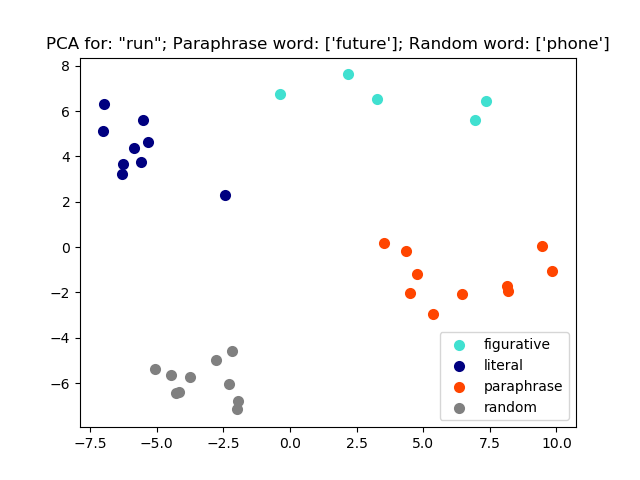
\includegraphics[height=5.5cm]{Paper/pair_id_23_fig_lit_para_rand.png}
\end{figure}


\section{Discussion}
The accuracy we achieved on idiom paraphrasing suggests that this task can be learned by BERT. However, our results are made suspect by the fact that there are some unusual patterns in our data that may be biasing our results, allowing BERT to ``cheat." Given that our \textit{combined} embedding paradigm achieved only 65\% accuracy on MRPC regardless of which BERT model we used, the fact that it achieves nearly 75\% accuracy on our data even without fine-tuning is somewhat suspicious. We suspect that this is due to our paraphrase sentence pairs having high structural overlap. Because only the section with the idiom is different in the paraphrase candidates and the rest of the sentence remains fixed, the result of subtracting one sentence embedding from the other will be composed entirely of the difference between the mean of the tokens for the idiom and the mean of the tokens for the text that replaced it. In effect, this means that the only semantic differences in our data are also the only actual differences, which may explain the success of the \textit{combined} sentence embeddings paradigm on our data. 

Manual inspection of the classifier outputs also points to the model's judgements being guided by structural overlap and other biases. As an example, for the model fine-tuned on the idiom data and the probing classifier trained on MRPC and tested on the idiom data, 45\% of false positives were found to contain all types of sentences while false negatives (3\% of the test data) were entirely composed of shorter samples, for which the substitution of a few words is more significant. For the best performing model which was fine-tuned, trained, and tested on the idiom data, the overall commonality seemed to matter: out of the pairs classified as false negatives, one third were idiomatic paraphrases and the other two thirds contained some abnormalities such as distributional oddities, unconventional spelling or grammar, or were incomplete sentence fragments.


That said, the performance of the CLS token embeddings follows a more reasonable trend and is likely to be more representative of BERT's treatment of idiom paraphrasing as a task. As Chart \ref{fig:accuracyByParadigm} shows, the CLS embedding from base BERT is nearly useless, the CLS embedding from BERT fine-tuned on MRPC performs better, and the CLS embedding from BERT fine-tuned on our idiom paraphrase data performs nearly identically to the \textit{combined} sentence embeddings. The discrepancy between \textit{cls} embedding paradigm performance and \textit{combined} sentence embedding paradigm performance in the first two cases suggests that whatever information is leading to our relatively high accuracies is not immediately available to BERT as it generates the CLS token, and the improved \textit{cls} performance when using the model fine-tuned on MRPC demonstrates that our data bears a significant degree of similarity to standard paraphrase tasks. Similarly, an experiment fine-tuning BERT on our data and training/testing the linear probe on MRPC achieves 72.8\% accuracy, also speaking to this overlap. Unfortunately, it is much harder to say whether the jump in \textit{cls} accuracy we see fine-tuning on our idiom data versus MRPC is a result of actually learning idiom paraphrasing as a task, or of BERT learning some heuristic particular to our dataset. A heuristic learned as a result of our data could similarly obscure the effects of training and testing on disjoint idiom data.

Finally, the question of whether or not the model's ability to understand paraphrases of a given idiom is substantially affected by that idiom's presence in training data likely remains open (see Chart \ref{fig:accuracyByDataSplit} in the appendix). For the best performing cases where we fine-tune on our idiom data there is a 4\% difference in accuracy. However, our dataset is sufficiently small that this relatively minor difference in performance could easily be accounted for by more challenging examples coincidentally being placed in test for the disjoint set. 


\section{Conclusion}

While it appears that we have successfully trained BERT to identify paraphrases containing idioms with nearly the same accuracy that it identifies normal paraphrases, we are reluctant to state this with certainty because time constraints prevented us from precluding the possibility that our data is biasing our results.

Overall, cosine similarity between sentence embeddings (produced by averaging word embeddings) appears not to be a good diagnostic for differentiating between paraphrases and non-paraphrases in sentences with idioms, nor correlated with our linear classifier's predictions. However, our word embedding similarity experiments suggest that contextualized word embeddings \textit{do} contain semantic information capable of differentiating use of a word in an idiom phrase from its use in a literal context.



\subsection{Future Work}

An obvious first step in improving this work would be attempting to recreate these results on a wider variety of data and to fix the quirks of our data addressed in the Discussion section. Even a comparison of our results to accuracy on paraphrase detection when the inputs are only the idiom and its paraphrase, neither with any sentence context, may shed light on the role that sentence context is playing in the comparison. Balancing the data taking into account linguistic factors such as the degree of compositionality, part-of-speech content, and frequency of the idiom as well as sentence length and syntactic structure could be another step to gain insights about the model's behavior.

There are also improvements to the probing methodology that could produce more results. Some results might look slightly different with a more standard linear probe, as opposed to the probe architecture that we ended up using.$^{\ref{probe-wrong-note}}$ Additionally, there are a wide variety of other ways  embeddings for the \textit{combined} paradigm could be produced. Sentence embeddings could be generated as a sum instead of an average, or produced from only a subset of the word embeddings. The input to the linear probe could be the sum, product, or even concatenation of the two sentence vectors instead of the difference between them. Experimenting with various methods of generating and combining sentence embeddings and how these changes affect performance is an area that we would have liked to spend more time on. 

Finally, an exploration of how the architecture of the final layers of BERT affects the results of fine-tuning could prove valuable. We used the Transformers library's to perform fine-tuning, which fine-tunes BERT using the CLS token exclusively \citep{Wolf2019HuggingFacesTS}. However, we would be very interested to see what kind of accuracy was possible if BERT was fine-tuned such that the input to the final linear classification layer were some combination of sentence embeddings, similar to our \textit{combined} embedding paradigm. 


\bibliography{anthology,acl2020}
\bibliographystyle{acl_natbib}

\newpage\phantom{blabla}
\newpage

\appendix \section{Supplemental Material}

\subsection{Idiom Paraphrase Dataset}\label{section:dataset}

To explore the effects of various parameters of the data, we produced splits of our data by size, origin, and train/test distribution, all of which had a 80/20\% train/test split. To examine the effect of the train/test distribution, we created datasets in which none of the idioms in our test set appear in the train set. This is to ensure that our experiment is testing performance on idioms generally, and not just memorizing those in the training set. To explore the effect of dataset size, we created sets of 2000 samples and 1000 samples from each of the following: MRPC, our randomly spilt dataset, and our dataset with no idiom overlap in train/test.
% we never speak about these datasets in the paper, they shouldn't be mentioned?
Finally, we created 2 datasets that are separated by the method of creation(automated and manual). 

Table \ref{tab:DataPropertiesTable} shows a summary of detailed information about the idiom paraphrase datasets created for the probing classification task.

Figure \ref{fig:accuracyByDataSplit} Shows results for accuracy using the random data split compared to the disjoint data split for a selection of models.

\begin{figure}[h]
    \includegraphics[width=8cm]{Paper/accuracyByDataSplit.png}
    \centering
        \caption{Accuracy by Data Split. \textit{Finetuned on Idioms} refers the random split of idiom data (blue bar) or the disjoint split (orange bar).}
    \label{fig:accuracyByDataSplit}
\end{figure} 

\begin{table*}[h]
\centering
\scalebox{.75}{
\begin{tabular}{|l|l|l|l|l|l|l|l|l|} \hline
\textbf \textbf{Dataset} & {Samples} & \textbf{Idioms} &  \textbf{Max freq} & \textbf{Min Freq} & \textbf{Max len} & \textbf{Min len} & \textbf{Avg s. len} & \textbf{Avg p. len} \\ \hline
Random Idiom Split (train) & 1600 & 214 &  64 & 2 & 93 & 4 & 21.7 & 20.8\\ \hline
Random Idiom Split (test) & 400 & 154 &  16 & 1 & 93 & 4 & 21.6 & 20.5\\ \hline
Disjoint Idiom Split (train) & 1600 & 185 &  80 & 4 & 93 & 4 & 21.6 & 20.7\\ \hline
Disjoint Idiom Split (test) & 400 & 30 &  68 & 4 & 93 & 4 & 21.6 & 20.7\\
\hline

 Total& 2000 & 215 &  80 & 4 & 93 & 4 & 21.6 & 20.8\\ \hline
\end{tabular}}
\caption{Properties of the training and test datasets. Max and min freq represent the number of times the most and least common idioms occur in the data; similarly with max and min len but for sentence length. The final two columns are average lengths for the sentences with idioms and their paraphrases, respectively.}
\label{tab:DataPropertiesTable}
\end{table*}

\subsection{Linear Probe Hyperparameters}\label{section:probehyper}
Through experimental fine-tuning, we settled on the following hyperparameters: a batch size of 64 for extracting embeddings via BERT, a learning rate of \(e^{-6}\), an epoch count of 10,000, and a fixed random seed. Note that our learning rate, epoch count, and random seed are all strictly hyperparameters for training the linear probe and have no affect on BERT. Our low learning rate was intended to compensate for differences in learning between different embedding paradigms, and the high epoch count was a function primarily of two things: our low learning rate, and our use of batch gradient descent instead of stochastic (due to our small dataset).

\subsection{Word Embedding Usage Cosine Similarity}\label{section:cosinesimdiff}

This table further illuminates the similarity advantage among idiom v. idiom usage pair cosine similarity over idiom v. literal usage pairs by showing the average \textit{increase} in the idiom v. idiom cosine similarity scores over idiom v. literal usages.

\vspace{1mm}
\scalebox{0.94}{
\resizebox{\columnwidth}{!}{\begin{tabular}{|l|l|}
\hline
Model &  Average difference \\
\hline
\textit{bert-base-uncased} & 0.2474 \\
\textit{bert-large-uncased} & 0.1920 \\
MRPC fine-tuned & 0.1706  \\
idiom paraphrase data fine-tuned  & 0.2728  \\
\hline
\end{tabular}}}


\subsection{PCA Visualization Example\footnote{All of the PCA visualization images for each run are available in their corresponding output folder in our Github repo \href{https://github.com/spacemanidol/AnalyzingNeuralLanguageModelsGroup1/tree/master/vector_similarity/output}{here}. We also present them in this \href{https://github.com/spacemanidol/AnalyzingNeuralLanguageModelsGroup1/blob/master/vector_similarity/run_vector_similarity_words_comparison.ipynb}{Jupyter Notebook} for easier navigation/comparison.}}\label{section:pcaviz}
For illustration, below are the PCA visualizations generated for a randomly selected idiom phrase group: the ``bite the bullet" data group (using the non fine-tuned \textit{bert-base-uncased} to calculate word embeddings).

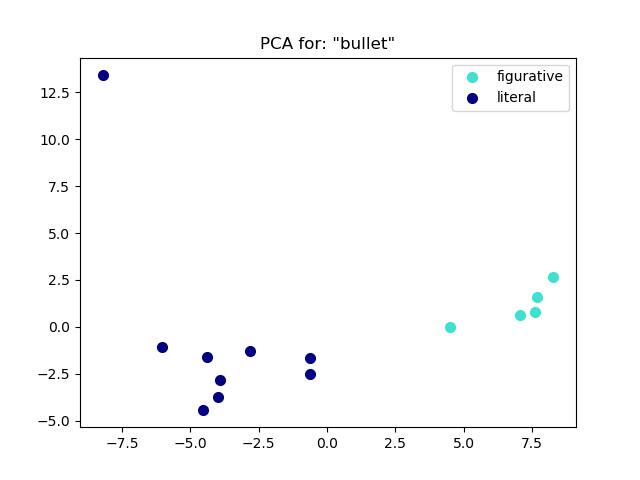
\includegraphics[height=6cm]{Paper/pair_id_21_fig_lit.png}
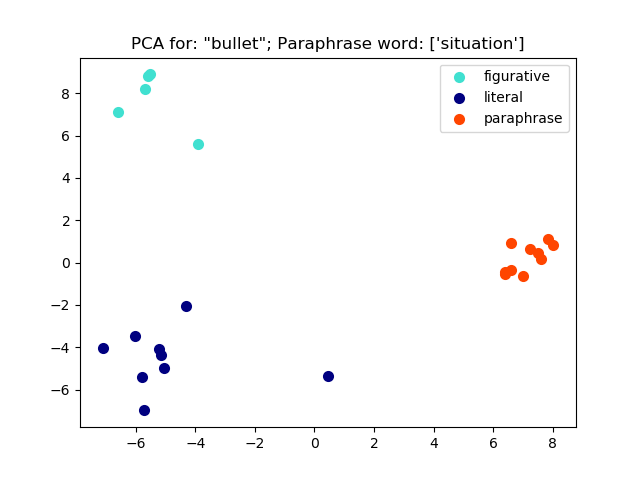
\includegraphics[height=6cm]{Paper/pair_id_21_fig_lit_para.png}
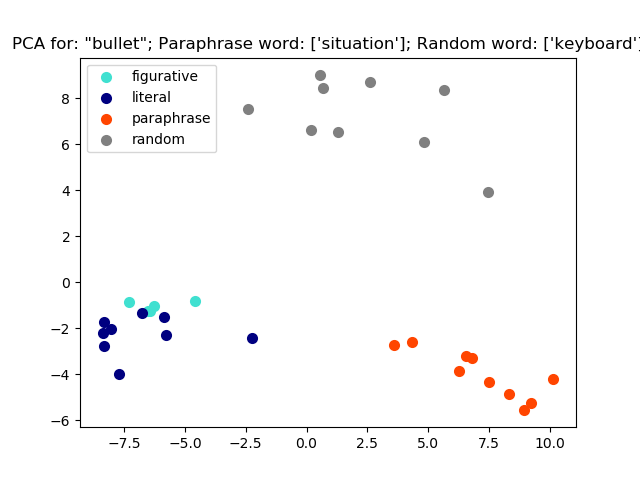
\includegraphics[height=6cm]{Paper/pair_id_21_fig_lit_para_rand.png}




Figure \ref{pcacat} shows a randomly selected visualization from the non-fine-tuned \textit{bert-large-uncased} model trial (embeddings for the word ``cat'' used literally and used as part of the idiom ``let the cat out of the bag," and for the paraphrase word ``secret"). Figure \ref{catmrpc} shows the same idiom phrase pair data from the model trained on MRPC.


\subsection{PCA Visualization of Base BERT versus Fine-tuned on MRPC}\label{section:pcamrpc}

\begin{figure}[h]
\caption{Non-fine-tuned \textit{bert-large-uncased}}
\label{pcacat}
\includegraphics[height=5.5cm]{Paper/pair_id_19_fig_lit_para_rand_bert_large.png}
\end{figure}

\newpage

\begin{figure}[h]
\caption{Model fine-tuned on MRPC}
\label{catmrpc}
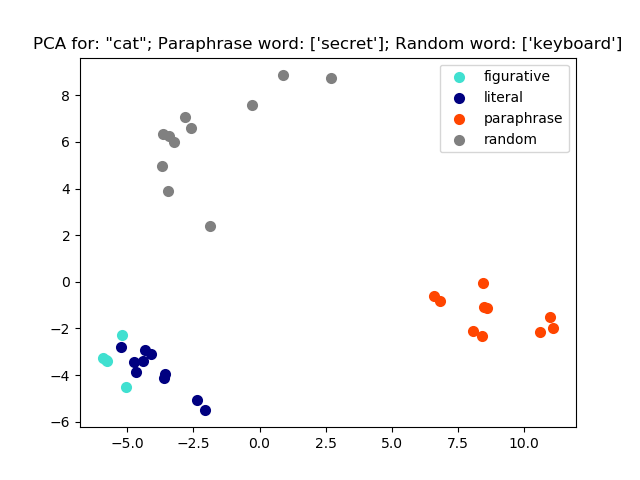
\includegraphics[height=5.5cm]{Paper/pair_id_19_fig_lit_para_rand.png}
\end{figure}


\subsection{Additional Data}

For the sake of completeness, we have included some additional information about our dataset and linear probe/fine-tuning experiments beginning on the next page.



\begin{table*}[h]
\caption{Average Cosine Similarity for Linear Classifier Experiments}
\label{tab:AvgCosineSimLinearClass}
\scalebox{.65}{
\begin{tabular}{|l|l|l|l|l|l|l|l|l|}
\hline
\textbf{Fine-Tune Data} & \textbf{train data} & \textbf{test data} & \textbf{True Positives} & \textbf{True Negatives} & \textbf{False Negatives} & \textbf{False Positives} & \textbf{All Paraphrases} & \textbf{All Non-Paraphrases} \\
\hline
Non Fine-Tuned & MRPC & MRPC & 0.9236 & 0.8474 & 0.8897 & 0.8865 & 0.9225 & 0.8810 \\
\hline
Non Fine-Tuned & Idiom & Idiom & 0.9283 & 0.9435 & 0.9532 & 0.9366 & 0.9334 & 0.9420 \\
\hline
MRPC & Idiom & Idiom & 0.9299 & 0.8486 & 0.8840 & 0.8928 & 0.9273 & 0.8852 \\
\hline
MRPC & MRPC & MRPC & 0.9310 & 0.9489 & 0.9685 & 0.9452 & 0.9398 & 0.9476 \\
\hline
Idiom & Idiom & Idiom & 0.9317 & 0.8652 & 0.8393 & 0.9271 & 0.9267 & 0.9222 \\
\hline
Idiom & MRPC & MRPC & 0.8946 & 0.9382 & 0.9556 & 0.9204 & 0.9013 & 0.9350 \\
\hline
 &  & \textbf{overall average} & 0.9232 & 0.8986 & 0.9150 & 0.9181 & 0.9252 & 0.9188 \\
\hline
\end{tabular}
}
\end{table*}

\begin{table*}[h]
\centering
\caption{Results on Idiom Paraphrase Task.}
\label{tab:paraphraseResultTable_Appendix}
\scalebox{.65}{
\begin{tabular}{|l|l|l|l|l|l|l|} \hline
Fine-Tuning Data & Train Data & Test Data & Combined Accuracy & Combined F1 & CLS Accuracy & CLS F1 \\
\hline
Non Fine-Tuned & Idioms (Random Split) & Idioms (Random Split) & 74.25\% & 74.10\% & 52.50\% & 53.66\% \\
\hline
Non Fine-Tuned & Idioms (Disjoint) & Idioms (Disjoint) & 74.50\% & 73.98\% & 57.50\% & 56.19\% \\
\hline
Non Fine-Tuned & MRPC & Idioms (Random Split) & 52.00\% & 67.90\% & 53.75\% & 68.80\% \\
\hline
Non Fine-Tuned & MRPC & MRPC & 66.49\% & 79.25\% & 71.54\% & 80.43\% \\
\hline
MRPC & Idioms (Disjoint) & Idioms (Disjoint) & 71.00\% & 67.78\% & 67.50\% & 67.98\% \\
\hline
MRPC & Idioms (Random Split) & Idioms (Random Split) & 73.00\% & 72.73\% & 64.50\% & 63.78\% \\
\hline
MRPC & MRPC & Idioms (Random Split) & 53.25\% & 68.25\% & 50\% & 65.64\% \\
\hline
MRPC & MRPC & MRPC & 65.16\% & 77.94\% & 80.64\% & 85.50\% \\
\hline
Idioms (Random Split) & Idioms (Random Split) & Idioms (Random Split) & 78.50\% & 78.60\% & 77.75\% & 78.86\% \\
\hline
Idioms (Random Split) & MRPC & Idioms (Random Split) & 51.50\% & 67.78\% & 53\% & 68.35\% \\
\hline
Idioms (Random Split) & MRPC & MRPC & 65.45\% & 78.62\% & 72.81\% & 81.26\% \\
\hline
Idioms(Disjoint) & Idioms (Disjoint) & Idioms (Disjoint) & 74.50\% & 72.87\% & 77.75\% & 80.09\% \\
\hline


\end{tabular}
}
\end{table*}



\begin{figure*}[h]
    \includegraphics[width=15cm]{Paper/accuracyByEpoch.png}
    \centering
        \caption{Accuracy by Epoch shown for two fine-tuned models. Both models trained and tested on idiom data.}
    \label{fig:accuracyByEpoch}
\end{figure*} 



\begin{table*}[h]
\centering
\caption{Results of fine-tuning; F1 score by batch count. Recall that batch size was 8 for all fine-tuning.}
\label{tab:paraphraseFineTuneResultTable_Appendix}
\hspace*{-2cm}\scalebox{.50}{
\begin{tabular}{ | l | l | l | l | l | l | l | l | l | l | l | l | l | l | l | l | l | l | l | }
\hline
	& 100 & 200 & 300 & 400 & 500 & 600 & 700 & 800 & 900 & 1000 & 1100 & 1200 & 1300 & 1400 & 1500 & 1600 & 1700 & End \  \\ \hline
	MRPC(Train 4076,Test 1726) & 0.8299 & 0.8491 & 0.8729 & 0.8689 & 0.8751 & 0.8811 & 0.8736 & 0.8769 & 0.8641 & 0.8756 & 0.8717 & 0.8691 & 0.8713 & 0.87 & 0.8713 & 0.8728 & 0.8731 & 0.8731 \\ \hline
	MRPC(Train 1600, Test 400) & 0.8391 & 0.8400 & 0.8242 & 0.8252 & 0.8400 & 0.9313 & 0.8321 & \  & \  & \  & \  & \  & \  & \  & \  & \  & \  & \  \\ \hline
	MRPC(Train 800, Test 200) & 0.8346 & 0.8544 & 0.8464 & 0.8541 & \  & \  & \  & \  & \  & \  & \  & \  & \  & \  & \  & \  & \  & \  \\ \hline
	Idioms Random(Train 1600, Test 400) & 0.7597 & 0.8435 & 0.8466 & 0.8305 & 0.8144 & 0.8204 & 0.8195 & \  & \  & \  & \  & \  & \  & \  & \  & \  & \  & \  \\ \hline
	Idioms Random(Train 800, Test 200) & 0.7699 & 0.7511 & 0.7571 & 0.73 & \  & \  & \  & \  & \  & \  & \  & \  & \  & \  & \  & \  & \  & \  \\ \hline
	Idioms DevUnique(Train1600, Test 400) & 0.7835 & 0.8355 & 0.8123 & 0.7937 & 0.7909 & 0.8018 & 0.8018 & \  & \  & \  & \  & \  & \  & \  & \  & \  & \  & \  \\ \hline
	Idioms DevUnique(Train800, Test 200) & 0.6813 & 0.8161 & 0.7372 & 0.7751 & \  & \  & \  & \  & \  & \  & \  & \  & \  & \  & \  & \  & \  & \  \\ \hline
	Train MRPC Test IdiomsRandom(Train 1600, Test 400) & 0.6811 & 0.6798 & 0.6550 & 0.6665 & 0.6778 & 0.6791 & 0.6780 & \  & \  & \  & \  & \  & \  & \  & \  & \  & \  & \  \\ \hline
	Train MRPC Test IdiomsDevUnique(Train 1600, Test 400) & 0.6700 & 0.6665 & 0.6479 & 0.6573 & 0.6562 & 0.6562 & 0.6562 & \  & \  & \  & \  & \  & \  & \  & \  & \  & \  & \  \\ \hline
	Train MRPC Test IdiomsRandom(Train 800, Test 200) & 0.6397 & 0.68 & 0.6755 & 0.6777 & \  & \  & \  & \  & \  & \  & \  & \  & \  & \  & \  & \  & \  & \  \\ \hline
	Train MRPC Test IdiomsDevUnique(Train 800, Test 200) & 0.6375 & 0.6633 & 0.6643 & 0.6633 & \  & \  & \  & \  & \  & \  & \  & \  & \  & \  & \  & \  & \  & \  \\ \hline
	Train MRPC Test IdiomsHandCrafted(Train 800, Test 200) & 0.6432 & 0.6843 & 0.6865 & 0.6865 & \  & \  & \  & \  & \  & \  & \  & \  & \  & \  & \  & \  & \  & \  \\ \hline
	Train MRPC Test IdiomsAutomated(Train 800, Test 200) & 0.5907 & 0.6121 & 0.6111 & 0.6077 & \  & \  & \  & \  & \  & \  & \  & \  & \  & \  & \  & \  & \  & \  \\ \hline
	Train IdiomsRandom Test MRPC(Train 800, Test 200) & 0.7963 & 0.7180 & 0.7066 & 0.6853 & \  & \  & \  & \  & \  & \  & \  & \  & \  & \  & \  & \  & \  & \  \\ \hline
	Train IdiomsDevUnique Test MRPC(Train 800, Test 200) & 0.5917 & 0.5527 & 0.4040 & 0.4849 & \  & \  & \  & \  & \  & \  & \  & \  & \  & \  & \  & \  & \  & \  \\ \hline
	Train IdiomsAutomated Test IdiomsHandCrafted(Train 800, Test 200) & 0.7062 & 0.7443 & 0.7477 & 0.7610 & \  & \  & \  & \  & \  & \  & \  & \  & \  & \  & \  & \  & \  & \  \\ \hline
	Train IdiomsAutomated Test MRPC(Train 800, Test 200) & 0.6912 & 0.5954 & 0.5636 & 0.5454 & \  & \  & \  & \  & \  & \  & \  & \  & \  & \  & \  & \  & \  & \  \\ \hline
	Train IdiomsAutomated Test IdiomsAutomated(Train 800, Test 200) & 0.7953 & 0.9951 & 0.9952 & 1 & \  & \  & \  & \  & \  & \  & \  & \  & \  & \  & \  & \  & \  & \  \\ \hline
	TrainIdiomsHandCrafted( Test IdiomsHandCrafted(Train 800, Test 200) & 0.9231 & 0.9556 & 0.9648 & 0.9567 & \  & \  & \  & \  & \  & \  & \  & \  & \  & \  & \  & \  & \  & \  \\ \hline
	TrainIdiomsHandCrafted( Test MRPC(Train 800, Test 200) & 0.7840 & 0.7853 & 0.7776 & 0.7828 & \  & \  & \  & \  & \  & \  & \  & \  & \  & \  & \  & \  & \  & \  \\ \hline
	Train IdiomsHandCrafted( Test IdiomsAutomated(Train 800, Test 200) & 0.7218 & 0.7291 & 0.7332 & 0.7271 & \  & \  & \  & \  & \  & \  & \  & \  & \  & \  & \  & \  & \  & \  \\ \hline
\end{tabular}}
\end{table*}



\begin{figure*}[h]
\caption{Results of F1 for fine-tuning based on training sample seen}
\label{fig:F1FineTunedataset}
\includegraphics[height=7cm,  width=\linewidth]{Paper/datasetsize.png}
\end{figure*}
\begin{figure*}[h]
\caption{Results of F1 for fine-tuning based on dataset source}
\label{fig:F1FineTuneSource}
\includegraphics[height=7cm, width=\linewidth]{Paper/source.png}
\end{figure*}

\begin{figure*}[h]
\caption{Results of F1 for fine-tuning based on transfer tasks}
\label{fig:F1FineTunetransfer}
\includegraphics[height=7cm, width=\linewidth]{Paper/transferlearning.png}
\end{figure*}
\end{document}